\chapter{Presentación de los datos, Análisis, Discusión}

En algunas disciplinas, el capítulo Presentación de datos va acompañado del análisis o de la discusión de la información (\textit{Presentación y análisis de los datos}; \textit{Resultados y discusión}), en tanto que en otras, \textit{Presentación}, \textit{Análisis} y \textit{Discusión} son capítulos separados.
El objetivo de esta(s) parte(s) de la tesis es presentar los datos recabados y el análisis realizado a la luz de la bibliografía ya revisada. Se puede incluir la interpretación de los resultados (\textit{Discusión}) a partir del análisis de los datos, o también relacionarlos con estudios relevantes que se entienden pertinentes, aun si estos no se han consignado en los \textit{Fundamentos teóricos}, ya que se entiende que al analizar los datos pueden aparecer algunos que no se enmarcan teóricamente o que no se explican en el encuadre teórico o en estudios ya existentes.

Ahora a modo de ejemplo mencionamos el símbolo de los números reales utilizando el comando \verb|\gls{}| \gls{Real} y el comando \verb|\glssymbol{}| \glssymbol{Real}. Otro ejemplo es mencionar el tensor simétrico de tensiones \gls{sigma}, o un valor escalar  \gls{alph} o un conjunto vacío \gls{emptyset}.

\newpage 


\section{Título de sección}

Ejemplo de tabla

\begin{table}[h!]
\centering
\caption{Leyenda de tabla.}
\label{tab:comp}
\begin{tabular}{|c|c|c|}
  \hline
  $t$ (seg) & $x$(t) & $y$(t)\\
  \hline
  1 & 0.0000 & 0.0001\\
  2 & 0.5000 & 0.2498\\
  3 & 1.0000 & 1.0000\\
  4 & 1.5000 & 2.2403\\
  5 & 2.0000 & 4.0010\\
  6 & 2.5000 & 6.2459\\
  \hline
\end{tabular}
\end{table}

Ejemplo de figura.

\begin{figure}[h!]
\label{fig:comp}
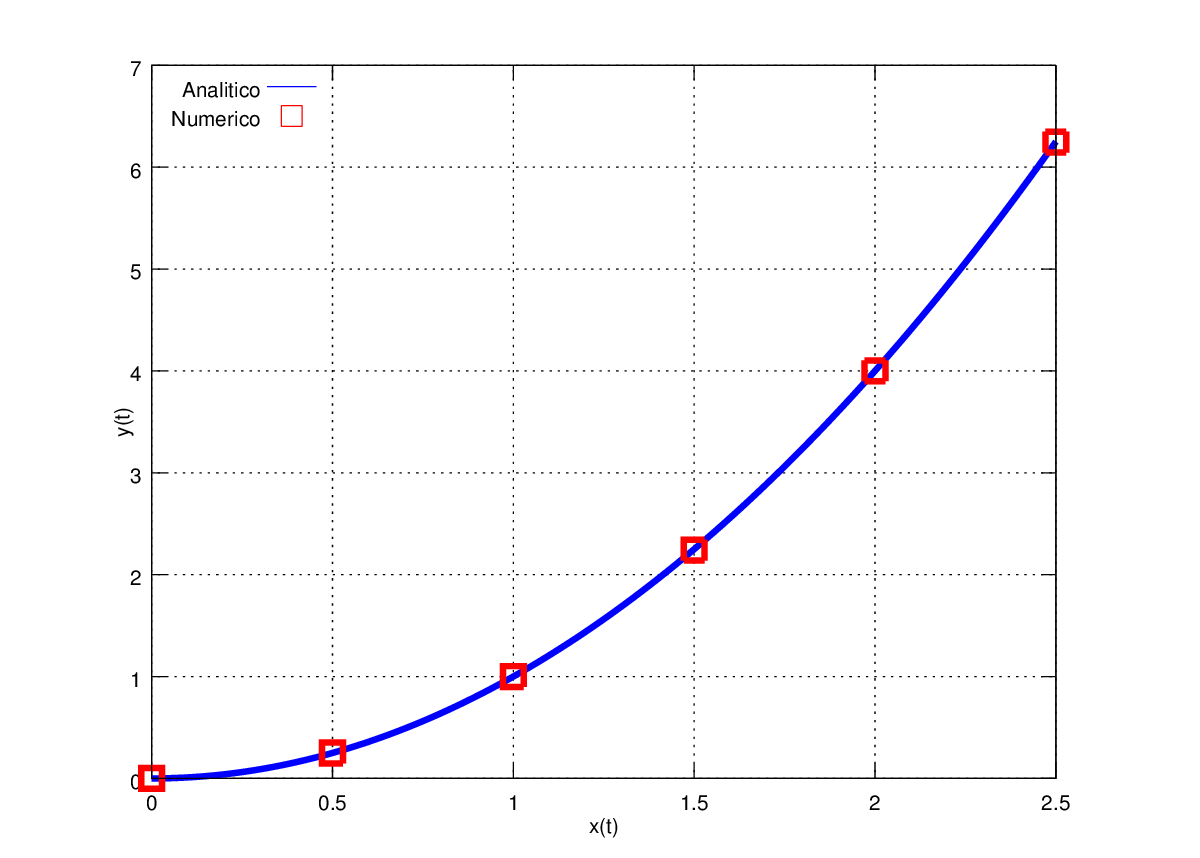
\includegraphics[width=.8\textwidth]{imagenes/chap4/x_vs_y}
\caption{Leyenda de figura.}
\end{figure}
Ejemplo de ecuación:
\begin{equation}
y(x)=x^2
\end{equation}


%\subsection{Conceptos y Medición}

%\subsubsection{Desempleo} 

El desempleo se entiende como personas que buscan trabajo remunerado activamente pero no logran obtenerlo. Según el \cite{INE2019} ``se considera como desempleado a toda persona que durante el período de referencia considerado (última semana) no está trabajando por no tener empleo, que lo busca activamente y está disponible para comenzar a trabajar ahora mismo. Por definición, también son desocupados aquellas personas que no están buscando trabajo debido a que aguardan resultados de gestiones ya emprendidas y aquellas que comienzan a trabajar en los próximos 30 días''. 
Su cálculo se realiza en función de la tasa de desempleo calculada por el INE y series trabajadas por parte del IECON.

%\subsubsection{Vacantes}

En la construcción del índice se tiene como base al Conference Board Help Wanted OnLine (HWOL) de EEUU, debido a que se observa \cite{Barnichon2010, Shimer2005} que es un proxy bastante confiable respecto del Job Openings and Labor Turnover Survey (JOLTS, calculado por el Bureau of Labor Statistics). Según el \cite{JOLTS} una vacante disponible debe cumplir 1)Una posición especifica exista 2)El trabajador pueda comenzar en no más de 30 días 3)El empleador busca activamente fuera del establecimiento la vacante.\footnote{Traducción propia} 


%\subsection{Fuentes de datos}
Los datos utilizados provienen prácticamente de una única fuente de datos, la misma es el diario El País, sección avisos laborales, ``El Gallito''. A partir de ella, construyen \cite{Rama1988} quién calcula un índice de vacantes desde 1978 hasta 1987 con base 100 en 1980\footnote{Utiliza también dos fuentes de datos construidas por el MTSS. Combina las 3 en un índice sintético de vacantes laborales} y \cite{Urrestarazu1997} que obtiene un índice de vacantes desde 1987 hasta 1995. Es Urrestarazu quién, une ambas series estimando la cantidad de avisos en el trimestre octubre-diciembre de 1986 e igualándola al valor del índice en dicho trimestre, con ello obtiene un índice de vacantes laborales desde 1978 hasta 1995, sin embargo, en su trabajo solamente se presentan los datos desde 1981-3. Dado que ambos índices fueron expresados en función de la Población Económicamente Activa (PEA) las mismas pueden ser combinadas.

El Centro de Estudios de la Realidad Económica y Social (CERES) construyó un índice de vacantes laborales llamado ``Índice CERES de Demanda Laboral'' (ICDL) con frecuencia mensual y desestacionalizado, desde marzo de 1998 hasta 2014 con base agosto 1998. Si bien no ha sido posible encontrar una nota metodológica precisa y detallada, si se han encontrado publicaciones \cite{Ceres2012} que detallan fue construido relevando información de solicitudes de trabajo publicados en la sección de clasificados de la prensa uruguaya, pero sin detallar la misma. Sin embargo, dada la preponderancia de los avisos clasificados publicados en El País, sección ``El Gallito'' la posibilidad que los mismos no hayan formado parte del análisis es nula. Bien pueden haberse agregado otras fuentes de información, siendo clasificados de otros diarios.

Dada la falta de información respecto al ICDL, se buscó contrastar al mismo con otras fuentes de información. Para ello se utilizaron los datos generados por \cite{Alma2011}, donde la base de datos fue facilitada por los autores. Con ella se construyó un índice de frecuencia anual, el cual se comparó con el ICDL también anualizado. Lo que se observa es un comovimiento de los mismos y una correlación del orden del 97\%. También se analizaron ambas series en tasas de crecimiento, mediante una transformación logarítmica y posterior diferencia, nuevamente ambas mostraron resultados similares con una correlación en torno al 90\%.

En este trabajo se han conseguido datos de avisos laborales publicados en el diario El País, sección ``El Gallito'' para 3 periodos de tiempo, 1995-1998, agosto 1998 y 2013-2018. El método de obtención de los dos primeros fue el mismo. Los datos fueron recabados manualmente revisando de forma exhaustiva las secciones de las publicaciones semanales de ``El Gallito'' guardadas en la Biblioteca Nacional. En el tercer caso, se obtuvo la base de datos de ``El Gallito'', la misma fue solicitada formalmente al Diario El País el cual accedió a compartir los datos, bajo estricto uso académico.

Las secciones de El Gallito son 5: masculino, femenino, servicio doméstico, otros trabajos pedidos y avisos destacados. Cada sección tiene su particularidad, masculino y femenino son las secciones que registran sistemáticamente mayor cantidad de avisos en el orden de 300-500 semanales, servicio doméstico entre 50-100, mientras otros trabajados pedidos es marginal e insignificante registrando 1-5 avisos. De crucial importancia resulta avisos destacados, ya que, si bien la cantidad de avisos publicados suelen ser 100-200 hay multiplicidad de avisos con gran cantidad de puestos solicitados. El hecho de que solo se hayan registrado los puestos de avisos destacados es debido a una restricción de tiempo y al mayor detalle que ofrecían dichas publicaciones.

Las series principales son 3, aunque existen algunas auxiliares donde se contabilizan cuantos avisos publicaron más de 10, 20, 30, 40 y 50 puestos. Se construye una serie de avisos, otra de avisos filtrados y finalmente una de puestos. La serie de avisos incluye a todas las secciones, y simplemente refiere a la cantidad de avisos publicados, por lo tanto, dicha serie es idéntica a la obtenida por Urrestarazu para los años 1989-1995. La serie avisos filtrados, tiene un solo cambio y es que los avisos destacados son filtrados. Por último, la serie puestos trabaja con el supuesto que los avisos publicados en todas las secciones salvo en avisos destacados son la cantidad de puestos pedidos, mientras que para avisos destacados se analizó cada aviso individualmente, algunos fueron filtrados y de los restantes se contaron los puestos requeridos.

Los avisos filtrados tenían las siguientes características: ofrecían invertir en algún negocio, se pedían corredores los cuales no se consideran empleados, solicitaban vendedores independientes, exigían realizar un curso previo en algún instituto, eran ventas por catalogo o bijou a consignación, solicitaban distribuidores, pedían viajeros no exclusivos Estos filtrados se realizaron solamente para los dos primeros periodos.

El primer periodo es desde septiembre de 1995 hasta junio de 1998, con datos obtenidos revisando las publicaciones semanales de forma exhaustiva. De allí se obtiene información de cantidad de avisos laborales para la sección masculino, femenino, servicio domésticos, otros trabajos pedidos y avisos destacados. Además se obtiene la cantidad puestos laborales para avisos destacados. El número de avisos obtenidos son cerca de 110.000, mientras la cantidad de puestos laborales de avisos destacados son aproximadamente 32.000. 

El segundo son los avisos laborales publicados en agosto de 1998, la metodología fue la misma que en el caso previo. La importancia de dicho mes, es que el ICDL tiene base agosto 1998. Por lo cual, era indispensable conocer dicho valor, el mismo fue de 4300 avisos publicados.

El tercero desde 2013-2018, contiene toda la información publicada en los avisos laborales a excepción de los nombres de empresas catalogados como reservadas.

Los datos mencionados pueden verse en la figura \ref{fig:vacantes}. En el cuadrante (a) tenemos los datos recolectados por \cite{Alma2011}, los mismos vienen se dividen entre los avisos propiamente (es decir, cada publicación) y la cantidad de puestos totales en dichos avisos (puntos negros), ambos muestran un comovimiento. En el cuadrante (b) tenemos los datos utilizados en \cite{Urrestarazu1997} desde 1980 hasta 1995, los mismos representan la cantidad de avisos totales en cada año. En el cuadrante (c) tenemos las series de puestos y avisos recolectadas en este trabajo, donde se evidencia una correlación elevada de las series. En el recuadro (d) se observa la comparación entre las series de ICDL y IECON medidas en tasa de crecimiento anual, las mismas evidencian una correlación de 0.9. Finalmente en el rectángulo (e) tenemos el ICDL para el periodo de 1998 hasta 2014 con frecuencia mensual y desestacionalizado.

%\begin{figure}[h!]
%	\centering
%	\begin{subfigure}[b]{0.4\linewidth}
%		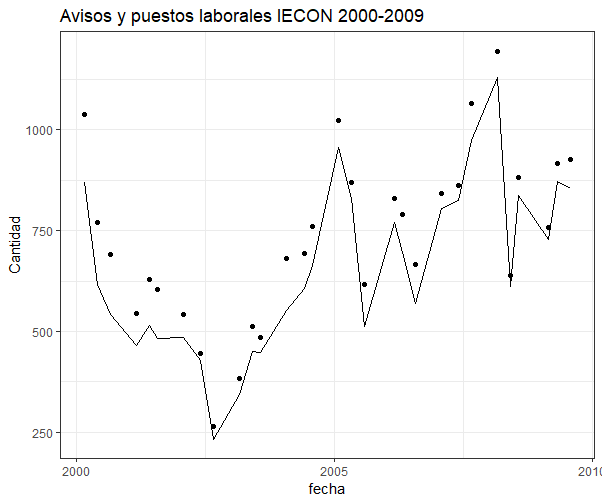
\includegraphics[width=\linewidth]{imagenes/chap4/iecon2000.png}
%		\caption{Avisos y Puestos IECON}
%	\end{subfigure}
%	\begin{subfigure}[b]{0.4\linewidth}
%		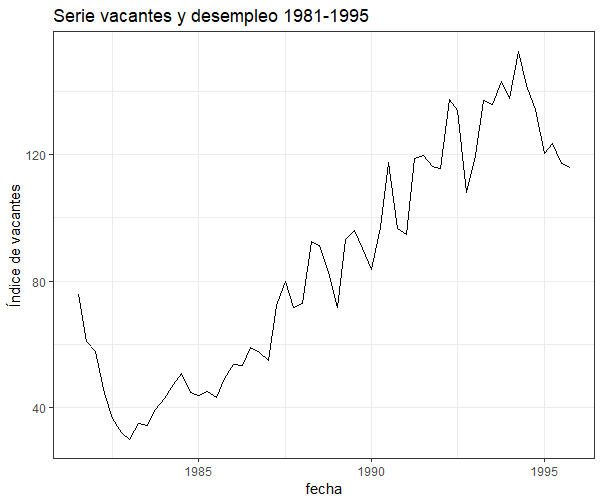
\includegraphics[width=\linewidth]{imagenes/chap4/VacantesUrrestarazu.png}
%		\caption{Vacantes Urrestarazu}
%	\end{subfigure}
%	\begin{subfigure}[b]{0.4\linewidth}
%		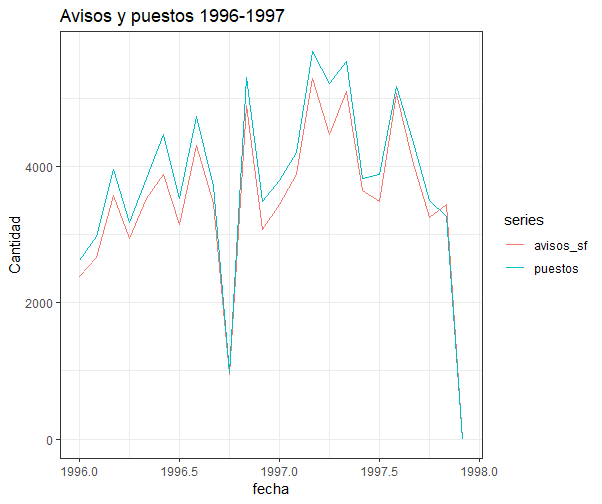
\includegraphics[width=\linewidth]{imagenes/chap4/MolinaAvisosyPuestos96.png}
%		\caption{Avisos recolectados 96-98}
%	\end{subfigure}
%	\begin{subfigure}[b]{0.4\linewidth}
%	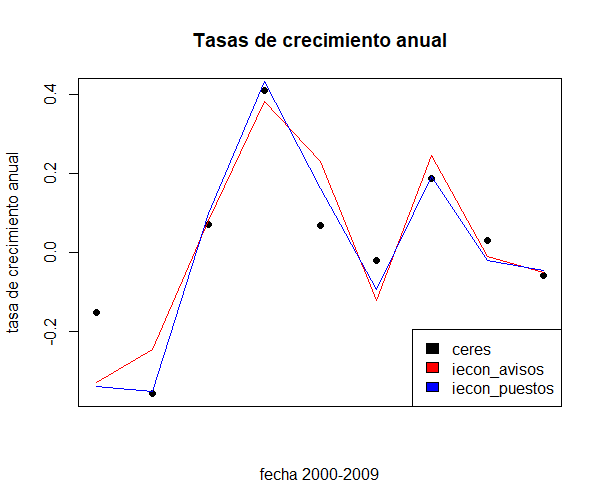
\includegraphics[width=\linewidth]{imagenes/chap4/CeresIECON2000.png}
%	\caption{Tasas crecimiento CERES-IECON}
%\end{subfigure}
%	\begin{subfigure}[b]{0.5\linewidth}
%		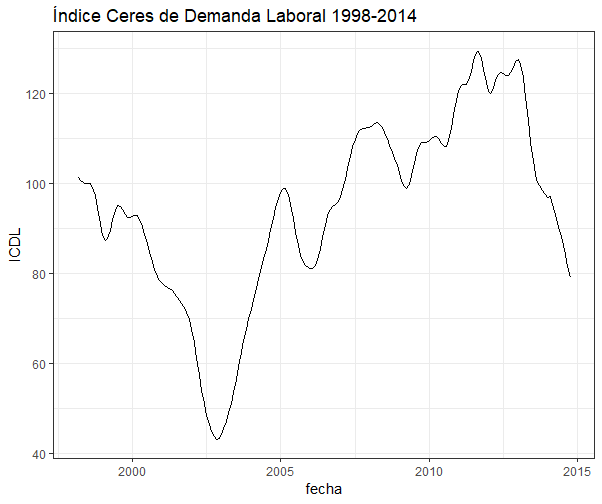
\includegraphics[width=\linewidth]{imagenes/chap4/ICDL98.png}
%		\caption{ICDL 1998-2014}
%	\end{subfigure}
%	\caption{Análisis de los datos obtenidos}
%	\label{fig:vacantes}
%\end{figure}

La serie de vacantes en proceso de construcción no esta exenta de críticas, las cuales vale destacar. La primera es que los datos solo permiten realizar un análisis para Montevideo, sin embargo, se encuentran sistemáticamente avisos laborales de otros departamentos del interior\footnote{Uruguay se compone de 19 grandes divisiones geográficas denominadas ``departamentos''. Por un lado esta Montevideo, y por el otro el resto de los 18 departamentos del país, lo que se denomina ``interior''.}, en especial de Maldonado y Canelones. Para el periodo recabado de 1995 a 1998 no se identifica cuantos avisos son y no son de Montevideo, sin embargo, si se logra obtener dicho número para el periodo de 2013-2018. En dicho caso los avisos publicados de otros departamentos oscilan en torno al 5\% del total publicaciones laborales. 

En segundo lugar, existe un claro sesgo hacia puestos laborales de baja calificación, lo cual se logra observar para el periodo 2013-2018 en base al análisis conjunto de la figura 2 y 3, donde se observa claramente que la mayor cantidad de avisos corresponden a puestos de auxiliar, técnico/especialista, ejecutivo comercial y peón. Esto va en linea con el resultado obtenido por \cite{Alma2011} para el periodo 2000-2010 utilizando la misma fuente de datos, quienes realizar un análisis pormenorizado de la información publicada en cada aviso laboral. Por lo cual, se supone que dicho sesgo también existe para el periodo 1980-1996.

%\begin{figure}[h]
%	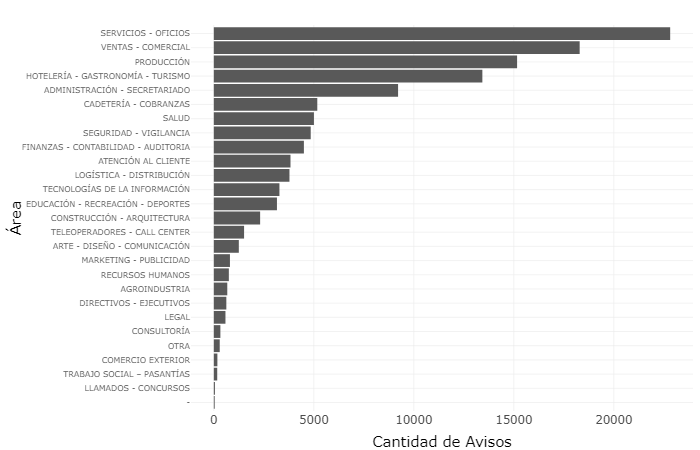
\includegraphics[width=\linewidth]{imagenes/chap4/newplot.png}
%	\caption{Cantidad de avisos laborales publicados en el diario El País, sección avisos laborales ``El Gallito'' entre 2013 y 2018. Los mismos son agrupados y ordenados de forma decreciente según el área en que se solicitan los avisos. El área, es una categoría propia del diario El País.}
%\end{figure}
%
%\begin{figure}[h]
%	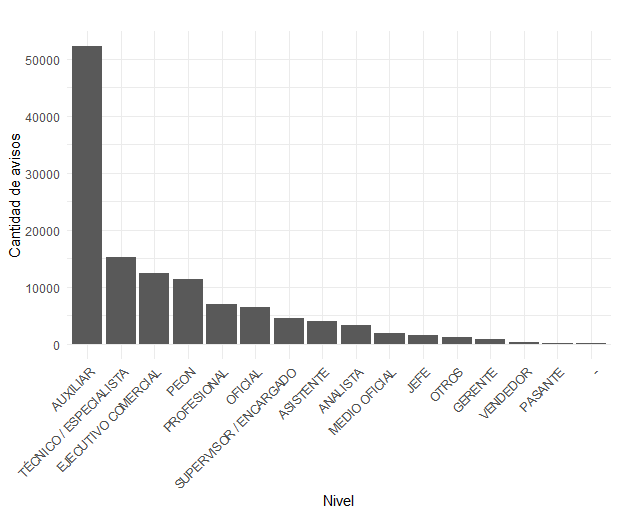
\includegraphics[width=\linewidth]{imagenes/chap4/gallito_nivel_2013_2018.png}
%	\caption{Cantidad de avisos laborales publicados en el diario El País, sección avisos laborales ``El Gallito'' entre 2013 y 2018. Los mismos son agrupados y ordenados de forma decreciente según el nivel jerárquico en que se solicitan los avisos. El nivel jerárquico, es una categoría propia del diario El País.}
%\end{figure}

En tercer lugar, la existencia de informalidad es una característica propia de los países subdesarrollados a la cual Uruguay y en específico Montevideo no escapa. Ello se agrava para los años entre 1980 y 2005, debido a las graves crisis económicas de 1982 y 2001-2002. Claramente las vacantes laborales publicadas en la prensa no captan los puestos generados en la informalidad.

Por último, ``El Gallito'' ha sido al menos hasta 2000-2010 el lugar predilecto por las empresas para publicar sus avisos laborales. Es un hecho incuestionable, por lo cual tomarlo como una muestra representativa de avisos laborales formales para el departamento de Montevideo es razonable. Sin embargo, con la penetración de Internet y la creación de portales de anuncios laborales como ``buscojobs'', ``computrabajo'', ``neuvo'' y ``linkedin'', entre otros, la competencia en el mercado de publicaciones ha aumentando considerablemente, no quedando claro en la actualidad cual es la página que reúne la mayor cantidad de avisos. Por esta razón, la representatividad del gallito ha disminuido y ello debe ser tenido en cuenta en el análisis, al menos desde 2009-2010 en adelante, dada la inserción de ``buscojobs'', ``computrabajo'' en torno a los años 2006-2007.

%\subsection{Estadísticas Descriptivas}

%[Presentar estadísticas descriptivas de los datos. Gráficos de las series, y al ser series temporales análisis estadísticas básicas de las series tales como test de R.U, de Raíz estacional, desestacionalización,]